%  $Description: Author guidelines and sample document in LaTeX 2.09$
%
%  $Author: ienne $
%  $Date: 1995/09/15 15:20:59 $
%  $Revision: 1.4 $
%
%\documentclass[times, 10pt,twocolumn]{article}
\documentclass[conference,final]{IEEEtran}
\usepackage{latex8}
\usepackage{times}

% Users' option
\usepackage{amssymb}
\usepackage{amsmath}
\usepackage{graphicx}
\usepackage{epstopdf}
\usepackage{color}
\topmargin=0.001in
\usepackage{multirow}
\usepackage{booktabs}
\newif\ifdraft
\drafttrue

\renewcommand{\multirowsetup}{\centering}
\renewcommand{\arraystretch}{1.2}
\def\nyc{\centering}

\ifdraft
\newcommand{\fixme}[1]{ { \bf{ ***FIXME: #1 }} }
\newcommand{\jhanote}[1]{ {\textcolor{red} { ***Jha: #1 }}}
\newcommand{\Nkimnote}[1]{ {\textcolor{green} { ***Nkim: #1 }}}
\newcommand{\skonote}[1]{ {\textcolor{blue} { ***Jeff: #1 }}}
\newcommand{\athotanote}[1]{ {\textcolor{green} { ***athota: #1 }}}
\newcommand{\Jkimnote}[1]{ {\textcolor{red} { ***Jkim: #1 }}}
\newcommand{\yyenote}[1]{ {\textcolor{blue} { ***yye00: #1 }}}
\else
\newcommand{\jhanote}[1]{}
\newcommand{\Nkimnote}[1]{}
\newcommand{\fixme}[1]{}
\newcommand{\skonote}[1]{}
\newcommand{\Jkimnote}[1]{}
\fi

\makeatletter
\newcommand{\rmnum}[1]{\romannumeral #1}
\newcommand{\Rmnum}[1]{\expandafter\@slowromancap\romannumeral #1@}
\makeatother
% End of users' option

%\documentstyle[times,art10,twocolumn,latex8]{article}

%-------------------------------------------------------------------------
% take the % away on next line to produce the final camera-ready version
\pagestyle{empty}

\newcommand{\up}{\vspace*{-1em}}
\newcommand{\upp}{\vspace*{-0.5em}}
\newcommand{\ts}{$T_{s}$}


%-------------------------------------------------------------------------
\title{Efficient Runtime Environment for Coupled Multi-Physics Simulations: \\
Dynamic Resource Allocation and Load-Balancing}

% \author{Soon-Heum Ko, Nayong Kim, Joohyun Kim, Abhinav Thota, Shantenu Jha\\
% Center for Computation and Technology\\
% Louisiana State University, Baton Rouge, LA 70803, USA\\
% (sko,nykim,jhkim,athota1,sjha)@cct.lsu.edu\\
% % For a paper whose authors are all at the same institution,
% % omit the following lines up until the closing ``}''.
% % Additional authors and addresses can be added with ``\and'',
% % just like the second author.
% %\and
% % Dimitris Nikitopoulos\\
% % Mechanical Engineering Department\\
% % Louisiana State University, Baton Rouge, LA 70803, USA\\
% % meniki@lsu.edu\\
% \and
% Yaakoub El Khamra\\
% Texas Advanced Computing Center\\
% The University of Texas at Austin, Austin, Texas 78758, USA\\
% yye00@austin.mail.address\\
% }

\author{
 ~\\[-2em]
 Soon-Heum Ko$^{1}$, Nayong Kim$^{1}$, Joohyun Kim$^{1}$, \\ Abhinav Thota$^{1,2}$, Shantenu Jha$^{*1,2}$\\
 \small{\emph{$^{1}$Center for Computation \& Technology, Louisiana State University, USA}}\\
 \small{\emph{$^{2}$Department of Computer Science, Louisiana State University, USA}}\\
 \small{\emph{$^{*}$Contact Author}}\\
}

%\thispagestyle{empty}

\begin{document}

\maketitle

\begin{abstract}
  Coupled Multi-Physics simulations, such as hybrid CFD-MD
  simulations, represent an increasingly important class of scientific
  applications.  Often the physical problems of interest demand the
  use of high-end computers, such as TeraGrid resources, which are
  often accessible only via batch-queues. Batch-queue systems are not
  developed to natively support the coordinated scheduling of jobs --
  which in turn is required to support the concurrent execution
  required by coupled multi-physics simulations. In this paper we
  develop and demonstrate a novel approach to overcome the lack of
  native support for coordinated job submission requirement associated
  with coupled runs. We establish the performance advantages arising
  from our solution, which is a generalization of the Pilot-Job
  concept -- which in of itself is not new, but is being applied to coupled
  simulations for the first time.  Our solution not only overcomes the
  initial co-scheduling problem, but also provides a dynamic resource
  allocation mechanism. Support for such dynamic resources is critical
  for a load-balancing mechanism, which we develop and demonstrate to
  be effective at reducing the total time-to-solution of the
  problem. We establish that the performance advantage of using
  BigJobs is invariant with the size of the machine as well as the
  size of the physical model under investigation.  The Pilot-Job
  abstraction is developed using SAGA, which provides an
  infrastructure agnostic implementation, and which can seamlessly
  execute and utilize distributed resources.
\end{abstract}
\up\up


%-------------------------------------------------------------------------
\section{Introduction}

Coupled Multi-Physics simulation techniques are being increasingly
used to study many different physical phenomena spanning time and
length scales at different levels of
detail~\cite{Tai}~\cite{Watanabe}. These techniques have been used to
investigate phenomena from crack-propagation in materials, biological
systems as well as understanding multi-phase fluid flow in constrained
geometry.

In addition to the ``physics challenges'' of these Multi-Physics
coupled simulations, there exist interesting ``computational
challenges''. Probably the best known (and investigated) is the
challenge of simulating large and complex systems, leading to
simulations that require greater computational resources -- often
involving HPC resources. % and no longer working on dedicated PCs.
Parallelization helps individual codes address the computational
demand of large and complex systems, but incorporating two distinct
codes under the umbrella of a single tightly-coupled application (say
using MPI) is not without significant problems. For example, the two
codes can often have very different computational kernels (one could
be mesh-based, the other unstructured particle simulations) with very
different computational time-scales.

Here we will focus on the challenges arising from running
tightly-coupled simulations on production systems with batch-queues,
whereby it cannot be guaranteed that two separate jobs will execute
concurrently. Specifically we will consider the case of coupling a
Computational Fluid Dynamics (CFD) code and a Molecular Dynamics (MD)
code, where the communication is via the exchange of files and not
Unix pipes (see next section for details on the coupling).

% Users' account loss is inevitable in conventional queuing systems
% except when sufficient CPUs are idling,

Although not exactly tightly-coupled in the sense of MPI, viz., very
frequent and with an extreme sensitivity to latency in communication
delay, the CFD and MD codes communicate frequently, (e.g., the CFD
code conducts data exchange in every iteration) and thus they need to
run concurrently. Thus, without explicit support for co-scheduling, it
is unlikely that coupled CFD-MD simulations will run concurrently as
inevitably the first job to run will have to wait for the other to
follow.

% \jhanote{Place the following appropriately} Thus, the best way using
% conventional job submission system would be to find a site with
% sufficient resource pool and submit two jobs with the optimal number
% of processors according to the pre-test data on performance of each
% tool in that facility with the same problem size.

Another important challenge, especially for large-scale simulations is
the need for efficient load-balancing, taking into account the
individual application's performance. Even if the two simulations could
run concurrently, without explicit load-management/balancing support,
there is likely to be inefficient utilization of compute resources due
to load imbalance. As the performance of each simulation component
changes with computing resource and problem size, re-adjustment of
allocated resources to each task according to their performance is
required during the simulation. Interestingly, as we will show,
effective load-balancing of two independent but concurrently running
codes introduces the need for dynamic resource allocation, and the
same solution that we devise to overcome the concurrent scheduling
requirement/constraints of coupled jobs also supports the feature of
dynamic resource allocation. In contrast, if simulations were
submitted as independent jobs, changing resource (CPU) allocation to
address these changes is challenging -- as the change in resource
assigned to one is correlated with a change in resource assigned to
the other component.

%\athotanote{ the other 2 scenarios? we are yet to introduce the scenarios!?}
The Pilot-Job is just a container task where a number of sub-tasks can
run in a pre-defined schedule with the specified number of processors
whether or not they are coupled.  The dynamic resource allocation
capabilities of the Pilot-Job prove useful
%in the other two scenarios,
in our scenario of using multiple Pilot-Jobs on the single container task
%\skonote{editied:nay need correction next}
as well as when using load-balancing in the single-resource scenario.
Although the container-Job/Pilot-Job concept is not novel {\it per
  se}, we believe this is the first documented utilization of these
abstractions to perform coupled Multi-Physics simulations. We claim
that there several distinct advantages that arise as a consequence of
using Pilot-Jobs for Coupled Simulations: (i) obviates the need for a
co-scheduler while preserving performance, (ii) enables dynamic
resource allocation, which in turn is important for load-balancing
across coupled simulations.  But given the lack of system or
service-level support to address the challenges outlined above, there
is a need to address the solution at the application level. This paper
aims to provide novel solutions to the above problem using frameworks
that are in user (application) space.

We will provide details on how we implement our solution in Section \Rmnum{3},
but in a nutshell it is critical to mention that our solution and its
concomitant efficiency is not tied to either a specific application
set (or infrastructure) and is scalable and extensible. It is based
on SAGA (the Simple API for Grid Applications)~\cite{saga_web},
which is a high-level API which provides the basic functionality
required to implement distributed functionally -- both logically and
physically, in an infrastructure and middleware independent
fashion. SAGA enables creation of higher levels of abstraction,
such as a container-job or a Pilot-Job (which, as we will discuss, is
referred to as the BigJob~\cite{saga_royalsoc}). The SAGA-based
Pilot-Job is infrastructure neutral, unlike {\it all} other
Pilot-Jobs.

We begin the next section with an outline of the basic motivation for
coupled simulations and load balancing.  We will address this
fundamental question: Does the use of an infrastructure independent
container job assist in the time to solution of a coupled simulation? We
will determine that the answer is yes for a variety of different
resource utilization scenarios. In the simplest case of a coupled
simulation running on a single machine, we will establish that the
reason is the lowered waiting time typically associated with a larger
size request (on most queuing systems, for most commonly occurring load-factors).  As our experiments will show, performance improvement arise
from removing the need for scheduling the two-components separately
and in providing a single job-requirement to the queuing system.

%\jhanote{Next few paragraphs need attention}

%\skonote{Please leave unchanged on this section now:I'll take a look at that after changing section 5-B and 5-C}
% -------------------------------------------------------------------------
\section{Hybrid CFD-MD Approach: Understanding the Coupling,
  Communication and Load-Balancing Requirements}


The hybrid CFD/MD approach~\cite{Thompson},~\cite{Nie},~\cite{Yen} is
a simulation method which adopts the continuum hypothesis in capturing
macroscopic features of a flow-field and details atomistic
intermolecular interactions on interfaces of different materials by
using the MD approach. CFD can accurately predict flow properties on
conventional moderate/large size fluid domains, but is intrinsically
impossible to reflect characteristics of surrounding solid materials.
While MD can provide atomistic level resolution of interactions
between particles, it becomes computationally demanding as the size of simulated system grows. So, neither method is suitable for solving a mesh-scale fluid system where the viscous effect dominates the flow characteristics but macroscopic features are also worth capturing efficiently. The best solution would be, as can be seen in Fig.~\ref{Fig:Couette}, to
carry out the hybrid CFD/MD approach with which atomistic
interactions between solid elements and fluid particles near the wall
is simulated by MD and the far field flow is calculated by CFD.


% The hybrid approach provides a good balance between computational cost and atomistic details/resolution.

% when reduction of total computational cost and keeping the atomistic
% details are equivalently demanded.

% A scientific problem that can be effectively tackled by the hybrid
% CFD/MD approach would be, for example, the simulation of a flow-field
% where the viscous effect of solid boundary is so dominant that the
% length scale required becomes significantly larger than the typical
% size of a system conducted by the conventional MD. Additionally,
% understanding of this fluid system near the wall is profoundly
% important but can be achieved only through atomistic molecular
% dynamics. One solution is, as is seen in Fig.~\ref{Fig:Couette}, to
% carry out the hybrid CFD/MD approaches with which atomistic
% interactions between solid elements and fluid particles near the wall
% is simulated by MD and the far field flow is calculated by CFD.

%%%%% FIGURE %%%%%
\begin{figure}
\centering
%\vspace{-1em}
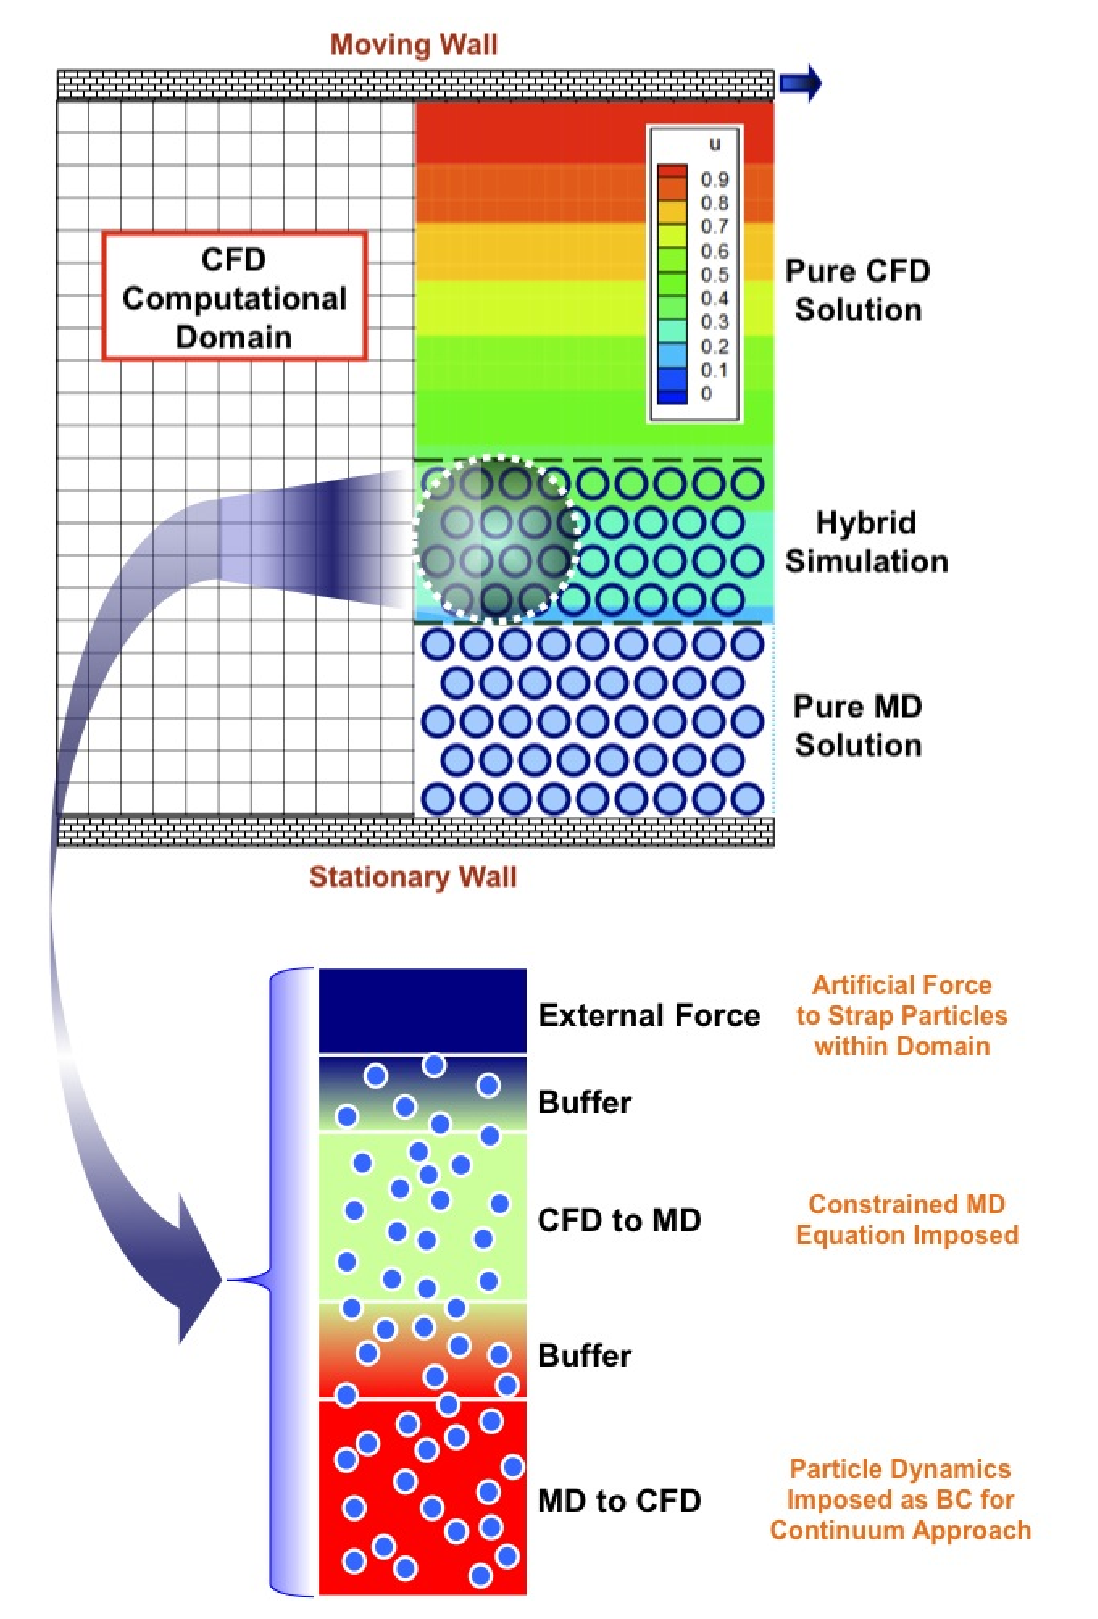
\includegraphics[scale=0.33]{fig1.eps}
%\linebreak
%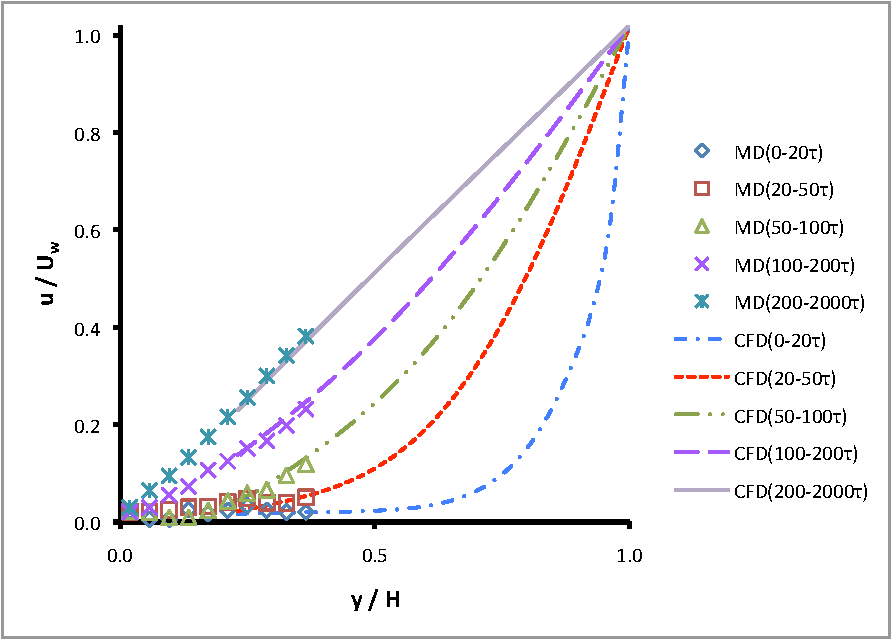
\includegraphics[scale=0.50]{Vel_Profile.PDF}
\caption{\small Schematic of CFD/MD Coupled Simulation of Channel Flow
  and the velocity profiles at different times}
\label{Fig:Couette}
\vspace{-1em}
\end{figure}
%%%%% FIGURE %%%%%

In this study, we built on the MPI version of the ``in-house''
incompressible CFD code~\cite{Lee} and the MPI version of
LAMMPS~\cite{LAMMPS} for MD. We did some modifications to these
application codes to implement hybrid schemes on each application
domain. In brief, the hybrid region where the coupling mechanism
between MD region and CFD region is executed comprises five
sub-regions. In the CFD boundary grid region positioned near the pure
MD region, velocities of particles obtained with MD are averaged and
used for boundary condition for the corresponding CFD computational
cells. The MD boundary zone is placed above the CFD boundary zone and
here the information on velocities from the CFD grid is imposed on
particles in the zone through dynamically constrained equation of
motion for MD. As illustrated in Fig.~\ref{Fig:Couette}, the coupling
mechanism is the key component for successful hybrid CFD/MD
simulations and our implementation follows the
literature~\cite{Nie},~\cite{Yen}.

% Between these zones, a buffer
% layer exists to avoid any harmful direct influences from one zone to
% another zone. The truncated and shifted Lennard-Jones potential is
% used for interactions of particles in MD simulation.

% To check the validity of the hybrid CFD/MD simulation, sudden-start
% Couette flow was employed that is similar to the test case used by
% O'Connell and Thompson~\cite{Thompson}.  The velocity profiles of
% hybrid approach are shown in the bottom of Fig.~\ref{Fig:Couette}. The
% line shows the velocity evolution which is solved by Navier-Stocks
% equations averaged over the given time intervals. MD results are shown
% as marks with same time intervals of CFD and overlap regions is
% indicated as both line and marks in the figure. These result is
% carried out for code validation of both CFD/MD and hybrid
% simulation. Good agreement between simulation results and analytical
% soluations.

As clearly indicated in Fig.~\ref{Fig:Couette}, the most prominent
computational challenge is how to run efficiently two separate stand
alone applications while efficiently conducting information exchange.
In other words, the time-to-solution is heavily dependent upon whether
a runtime environment can provide, (i) low collective-waiting times
(arising from batch queue wait times), and (ii) prevent an imbalance
in the time to reach the information exchange step between the two codes. The
imbalance arises due to difference in performance between two distinctly
heterogeneous applications, CFD and MD, resulting in an unavoidable
time gap between arrival times of CFD and MD for the exchange step. We
propose to address this using dynamical resource allocation mechanism
with a load-balancing mechanism. In that sense, our SAGA-based
framework provides a single efficient runtime environment for the
coupled simulation.

%\Nkimnote{ }
%-------------------------------------------------------------------------
\section{SAGA and SAGA-based Frameworks for Large-Scale and Distributed Computation}

The Simple API for Grid Applications (SAGA) is an API standardization
effort within the Open Grid Forum (OGF)~\cite{ogf_web}, an
international standards development body concerned primarily with
standards for distributed computing. SAGA provides a simple,
POSIX-style API to the most common Grid functions at a sufficiently
high-level of abstraction so as to be
independent of the diverse and dynamic Grid environments. The SAGA
specification defines interfaces for the most common Grid-programming
functions grouped as a set of functional packages
(Fig.~\ref{Fig:SAGA1}). Some key packages are:

\begin{figure}
%[!ht]
%\vspace{-1em}
 \begin{center}
     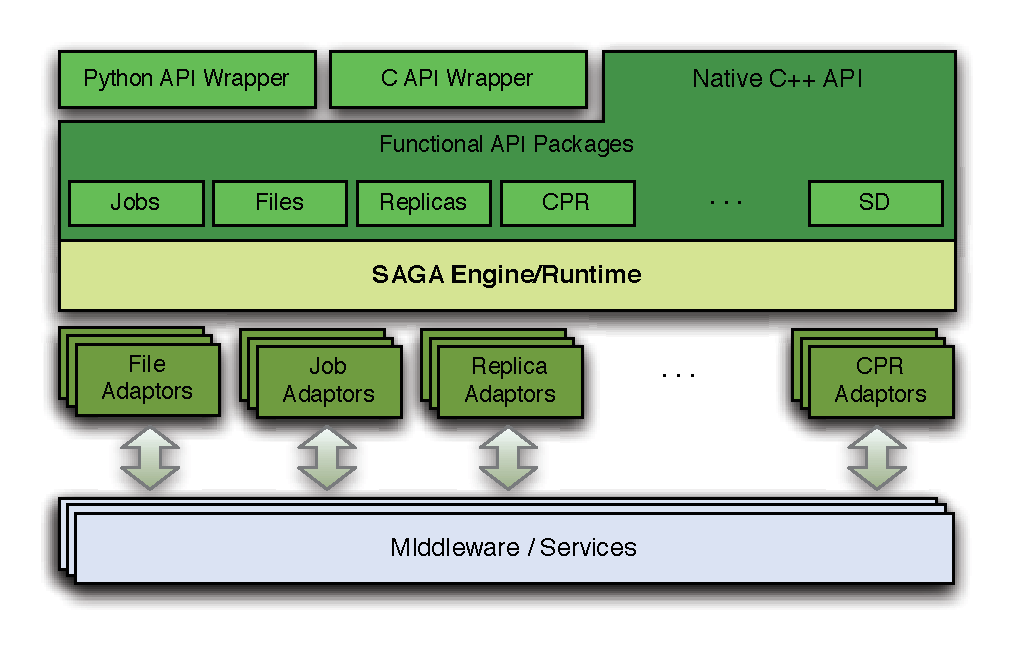
\includegraphics[width=0.40\textwidth]{stci_saga_figures-1}
 \end{center}
\caption{\small Layered schematic of the different components
  of the SAGA landscape. At the topmost level is the simple integrated API which provides the basic functionality for distributed computing. Our BigJob abstraction is built upon this SAGA layer using Python API wrapper} \label{Fig:SAGA1}
\vspace{-1em}
\end{figure}

\begin{itemize}
\item File package - provides methods for accessing local and remote
 filesystems, browsing directories, moving, copying, and deleting
 files, setting access permissions, as well as zero-copy reading and
 writing
\item Job package - provides methods for describing, submitting,
 monitoring, and controlling local and remote jobs. Many parts of
 this package were derived from the largely adopted
 DRMAA % ~\cite{drmaa_url}
 specification.
\item Stream package - provides methods for authenticated local and
 remote socket connections with hooks to support authorization and
 encryption schemes.
\item Other Packages, such as the RPC (remote procedure call) and Replica
 package
\end{itemize}


% \skonote{Introduction of PilotJob and BigJob (1 or 2 paragraphs) :
%   What is PilotJob, BigJob / what have been done so far and how
%   effective it was when using BigJob}

% \skonote{Joohyun, can you check this paragraph and improve it? In
%   this paragraph, I was going to talk about 'Structure and
%   Simulation Flow of BigJob Abstraction for Coupled Simulation'.}

Fig.~\ref{Fig:BigJob_Structure} shows the structure of BigJob and its
operation flow. When a BigJob is submitted to the remote resource, the
application manager monitors the status of this pilot-job through the
advert service. When resources are allocated to the BigJob, the
application manager allots the obtained resources to its sub-jobs and a
coupled simulation starts under the control of a multi-physics agent
in the remote resource. Advert service keeps on getting the status of
a pilot-job from the queuing system and the status of sub-jobs from
multi-physics agent and also delivers this information to the
application manager by a push-pull mechanism. The application manager
watches the status of sub-jobs and decides the next event when the
coupled simulation is finished. When one default BigJob is launched,
sub-jobs keeps running until final solution is achieved and the
manager quits the Pilot-Job at that time. In case multiple BigJobs
are submitted for the same simulation or if a load balancing function is
included, sub-jobs experience several restarts from their
checkpointing data, reflecting changed processor allocation to each
application. In the former case, resource allocation to each sub-job
follows a pre-defined map according to the number of BigJobs allotted
to the simulation; in the latter case, resource allocation to each
sub-job becomes dynamic according to its performance, as discussed
in the next section.

%%%%% FIGURE %%%%%
\begin{figure}
%\vspace{-1em}
\centering
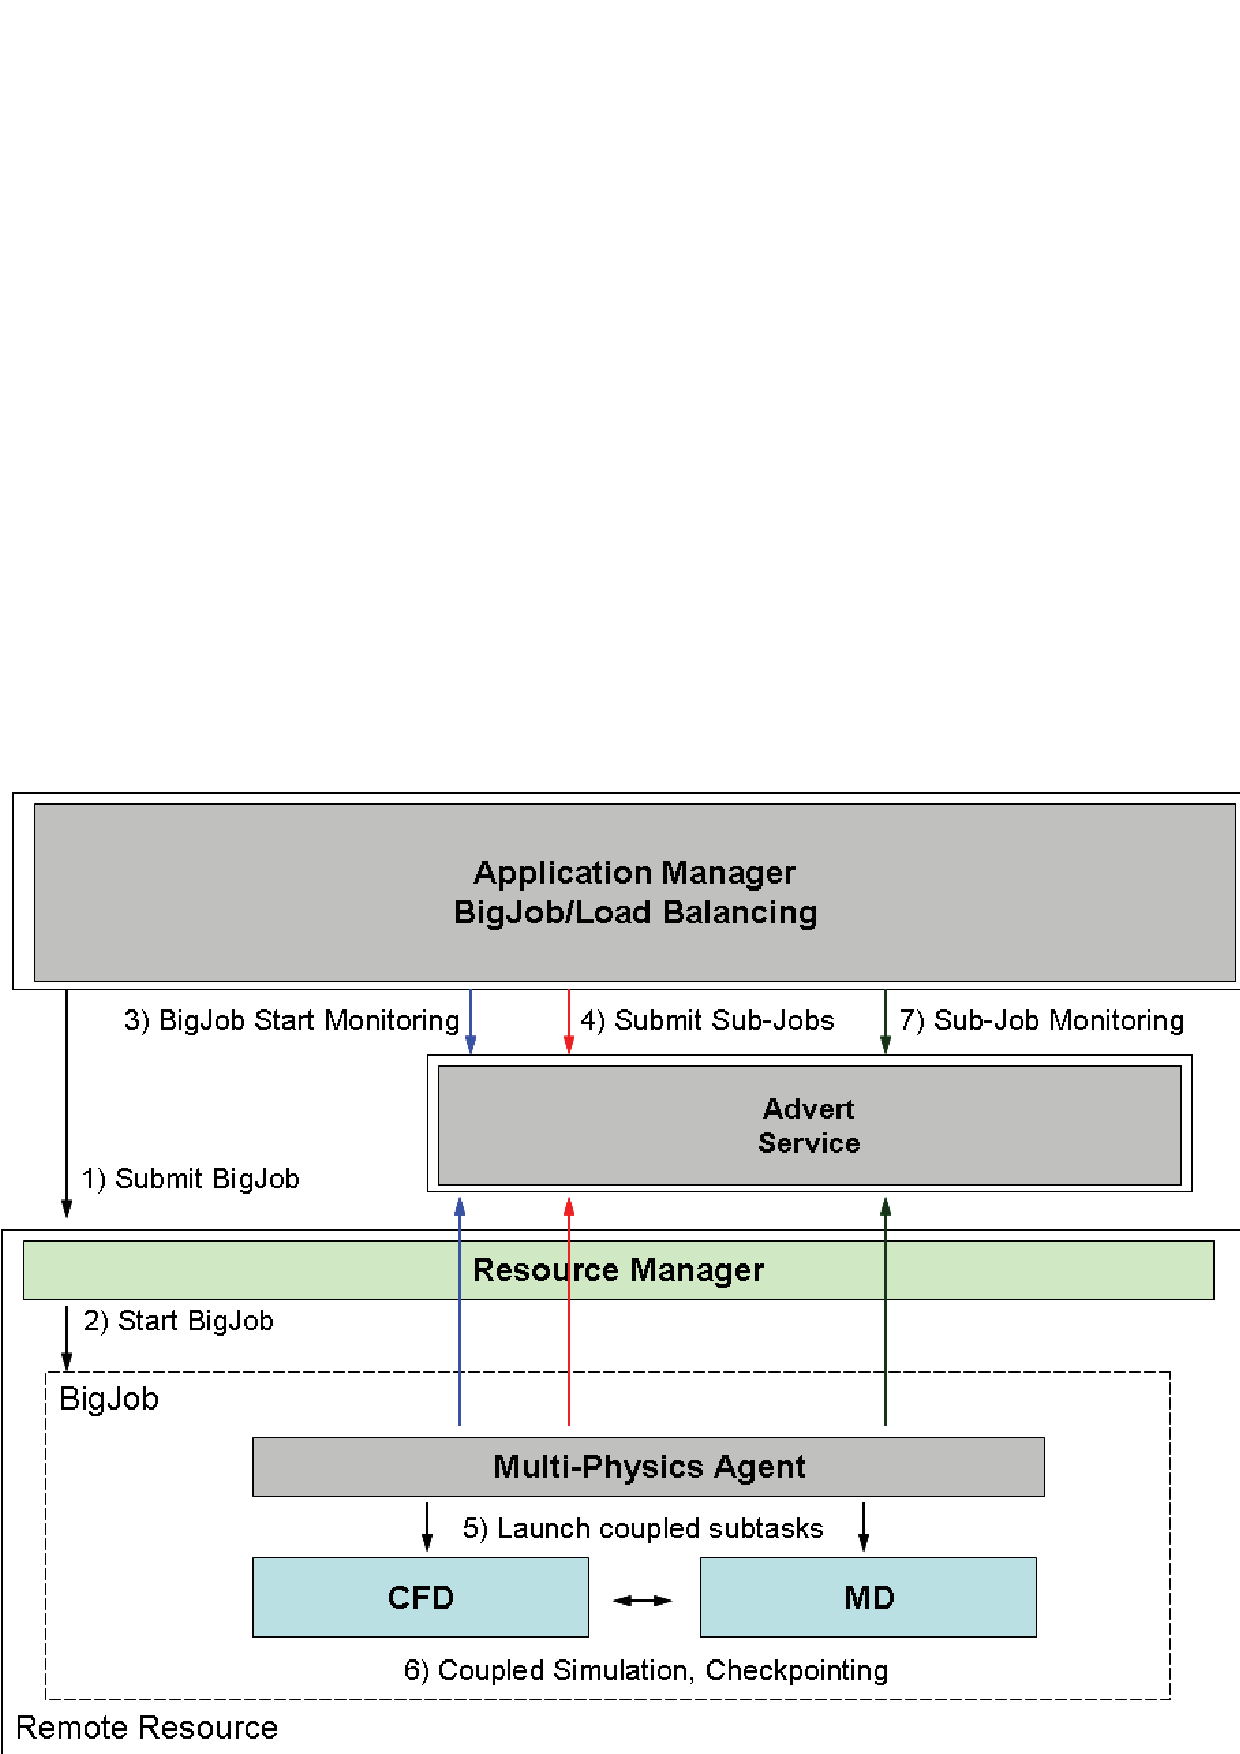
\includegraphics[scale=0.38]{Structure_of_BigJob}
\caption{\small Architecture of the Controller/Manager and Control
  Flow: Application manager is responsible for job management
  including BigJob and sub-job submission, their status monitoring
  functions. We implement a load balancing module, and migration
  service based on job information. Application agent system resides
  on each HPC resource and conducts job information gathering and also communicates with the application manager via the advert service}
\label{Fig:BigJob_Structure}
\vspace{-1em}
\end{figure}
%%%%% FIGURE %%%%%

%-------------------------------------------------------------------------
\section{Load Balancing for Coupled Multi-Physics Simulation}

The flexibility to re-distribute resources (processors) to the individual task does not imply efficient utilization. This is the responsibility of a load-balancer (LB). We will discuss the implementation and algorithm of this LB; it is important to mention that the LB functions in the context of the SAGA-BigJob framework.

Our LB is designed to propose the efficient resource allocation between tasks within a pilot-job. Conceptually, the load-balancing algorithm assigns more processors to a sub-task with greater runtime, until the two codes take the same wall-clock time between points when they communicate. Interestingly, our approach is very simple and the algorithm is independent of applications upon the predications of,
(1) each application code follows the ideal parallel efficiency.
(2) all processors in one node are assigned to one single task.

Let the computation time (between exchanges) of the two sub-jobs be $t_{CFD}$ and $t_{MD}$, and the number of processors assigned to each domain be $PE_{CFD}$ and $PE_{MD}$, respectively. Subscripts n and n+1 denotes the current and next stages. Based on assumption (1), total problem size of each application remains the same after resource re-allocation,

\vspace{-.2em}
\footnotesize
\begin{eqnarray}
W_{CFD}&=&PE_{CFD,n}\times t_{CFD,n}=PE_{CFD,n+1}\times t_{CFD,n+1} \nonumber \\
W_{MD}&=&PE_{MD,n}\times t_{MD,n}=PE_{MD,n+1}\times t_{MD,n+1}
\label{eq:SimTime_EachTask}
\end{eqnarray}
\normalsize

In spite of the re-allocation, the total number of processors utilized remains the same:

\vspace{-.2em}
\footnotesize
\begin{equation}
%\small
%\begin{center}
PE_{TOT}=PE_{CFD,n}+PE_{MD,n}=PE_{CFD,n+1}+PE_{MD,n+1}
%\end{center}
\label{eq:PECondition}
\end{equation}
\normalsize

Our objective is to reduce the computation time of a sub-job to the point until the two application components show the same computation between the exchange points, i.e., $t_{CFD,n+1} = t_{MD,n+1}$. From Equation~\ref{eq:SimTime_EachTask} and Equation~\ref{eq:PECondition} an optimal number of processors distributed for the CFD subtask would be:

\vspace{-.2em}
\footnotesize
\begin{eqnarray}
PE_{CFD,n+1} & = & \frac {W_{CFD}} {(W_{CFD} + W_{MD})} \times PE_{TOT}
\end{eqnarray}
\normalsize

The MD simulation (sub-job) will follow a similar expression.  The optimal processor distribution from above equation will return a non-integer value. Also, under the second assumption (which is the policy of many supercomputing centers), any load-balancing determined as above, will proceed in discrete values expressed as the multiples of the number of CPU cores in a node. We choose the nearest discrete number to our load balancing as the optimal number of processor on each application.

The load balancing function is deployed on the BigJob application manager and it operates as follows. Application codes are set up to have several restarts from its checkpointing data until the completion: application manager promotes these launch/re-launches of coupled sub-tasks. At the end of each simulation loop, the LB measures the best resource allocation between tasks based on applications' performance data. Changed resource allocation is applied at the next launch of application codes. By iteratively applying the LB, the resource allocation between coupled sub-tasks can gradually converge to a steady solution, even in cases application codes do not follow ideal parallelism.

For the efficient functioning of the LB, application codes need to be able to restart from their checkpointing data effectively. Also, application codes should be equipped with generalized domain partitioning routine to run a simulation with any number of processors, without harming their parallel efficiency a lot. Finally, they shall be able to produce their performance data, by checking wall-clock time between inter-domain data exchange.


%-------------------------------------------------------------------------
\section{Dynamic Resource Allocation for Coupled Simulations:
  Experiments and Analysis}

In Section  \Rmnum{2}, we outlined the challenges of running a coupled
multi-physics simulation using conventional queuing systems as the following: (i)
Difficulty of starting multiple applications concurrently; (ii)
Inability to balance the load among domains, and (iii) Fixed number of
allocated resources throughout the simulation. To address these
challenges we use the BigJob abstraction with a load balancing (LB) module
for dynamic resource allocation.

We outline three possible scenarios. In the first scenario, a single
BigJob is utilized to run the coupled simulations, with and without LB
(denoted as $S1_{LB}$ and S1 respectively) redistributing resources
based upon their individual performance.  In the second scenario (S2)
there are two BigJobs, and although they are started together, most
often one BigJob starts before the other; to increase efficiency, both
coupled simulations start with whatever resources are available as
part of the first (to run) BigJob. When the second BigJob becomes
active, there is a dynamic redistribution of tasks, such that the
larger of the two sub-jobs is assigned the bigger BigJob. Variant of
the above, when the two BigJobs are on two different machines forms
the third scenario (S3). In the remainder of this section we discuss
the details of these three different Use Cases.


\subsection{Description of Experiments}

Figure~\ref{Fig:OneBJ_Flow} shows two different scenarios: the first
(leftmost) shows the time evolution of a coupled simulation executing
after using a conventional job submission (which we define to be
scenario S0), and the other using a BigJob. For S0, individual tasks
with resource requirements of $PE_{CFD}$ and $PE_{MD}$ respectively,
are independently submitted to the conventional queuing system and job
scheduler recognizes these coupled tasks as two distinct jobs. Thus,
they are start at different times on average, except when
coincidentally resources for both are available. In this case, both
tasks wait on the queue when no job is allocated, the first allocated
job idles to perform data exchange with its counterpart; the actual
simulation executes only after both jobs are running/allocated. On the
other hand, for scenario S1, a BigJob of size $PE_{CFD}+PE_{MD}$ is
submitted to the queue, and coupled simulation directly starts when
the resource is assigned to this BigJob. Because of co-scheduling of
sub-jobs, a BigJob is free from long inactive mode which is frequent
in conventional job submission, while total runtime is the same if the
resource distribution to sub-jobs is identical. However, eliminating
inactive mode in of itself does not guarantee a reduction in the total
runtime, because a larger allocation may result in a greater queue
waiting time than two simulations requesting smaller number of
processors each (but the total being the same). The same situation can
arise for the load-balanced case with one BigJob.
Figure~\ref{Fig:TwoBigJobs} illustrates scenarios S2 and S3 -- whereby
2 BigJobs are submitted as opposed to 1 BigJob. In S2 both BigJobs are
on the same machine, whilst in S3 they are on different machines.
Compared to S2, S3 is more likely to get assigned with the second BigJob faster, while the active runtime will increase a little due to the slower communication between sub-jobs in distributed resources.


%%%%% FIGURE %%%%%
\begin{figure}
%\vspace{-1em}
\centering
\includegraphics[scale=0.4]{Simulation_Time_of_One_BigJob.eps}
\caption{\small Comparison of dependencies encountered for coupled
  simulations submitted as conventional jobs (S0), to the scenario when
  using Pilot-Jobs. Here we use only 1 BigJob (S1). The conventional
  mode of submission experiences three phases based upon their queue
  state: (i) All jobs are waiting: ($t_1-t_0$); (ii) Inactive mode
  (where one job is waiting for another: $t_2-t_1$), and (iii) Active
  mode (running a coupled simulation: $t_f-t_2$). The Inactive stage,
  disappears when a coupled simulation runs within a BigJob, as an
  allocated BigJob distributes its resource to both sub-jobs.}
\label{Fig:OneBJ_Flow}
\vspace{-1em}
\end{figure}
%%%%% FIGURE %%%%%


%%%%% FIGURE %%%%%
\begin{figure}
%\vspace{-1em}
  \centering \includegraphics[scale=0.4]{Simulation_Time_of_Two_BigJobs.eps} \caption{\small
    Schematic comparing the distribution of simulations when 2 BigJobs
    are used. On the left side, both BigJobs are submitted to the same
    physical machine (S2); on the right side they are submitted to
    different (distributed) machines (S3). In both cases, coupled
    sub-jobs start running when the first BigJob is allocated at
    $t=t_1$; there is a resource reallocation when the next BigJob
    becomes available. When two BigJobs are allocated, each sub-job
    occupies a BigJob, and data exchange between jobs takes place
    across BigJobs.}  \label{Fig:TwoBigJobs}
  \vspace{-1em}
 \end{figure}

We investigate a simple couette flow (Fig.~\ref{Fig:Couette}) as the
representative physical problem, to validate the performance gains and
resource flexibility of above scenarios.  The current flow system is
composed of 62,400 mesh points (CFD) and 23,188 particles (MD).  In
order to reach convergence, the coupled simulation runs for a physical
time of 2500$\tau$, which is the time unit related to the
characteristics of molecules. This is equivalent to 25,000 CFD
iterations and 500,000 MD integration steps. During the simulation,
both codes components update their boundary values by exchanging their
numerical data via files, once every 10 $\tau$. This leads to 250
synchronization steps between two simulation components over the
course of a single simulation run. For a rigorous test of a load
balancer, larger coupled simulation task (which has 150 times more
workload on CFD domain and 50 times on MD) also has been experimented. Total iterative loop is split into five launch/re-launch stages (25 times in larger simulation) after an application-level checkpointing, to facilitate the load balancing between sub-jobs or more BigJob allocations.

Evaluation of the effectiveness of BigJob as a job-submission
mechanism, requires carefully controlled experiments over different
processor requests and different wall-time limits with varying system
conditions.  To understand the queue waiting time of job submissions
and analyze the variation of waiting time with system's conditions
under similar or controlled conditions, we define the load-factor as
the ratio of the number of active nodes to the total number of nodes
on the machine. We determine the effect of load-factor on queue
waiting time by submitting a number of experiments to the resources
and monitoring the variance of load-factor at the submission and at
the allocation time. Our experiments include multiple job submissions
ranging from 8 to 64 px (processors) with wall-time limit from 1 to 12
hr (hours). This waiting time issue is also discussed by simulating above
coupled simulations, in a way of submitting a BigJob and two
conventional jobs concurrently and counting total waiting time in both
cases. Both small and large simulations are conducted using 64
px for a coupled task and wall-limit time is set to be either
6 hr or 24 hr, depending on their computation times.

Simulations used to validate and determine the performance measures
were conducted on supercomputing resources on TeraGrid machines
(62,976 cores Ranger), shared TeraGrid-LONI (Louisiana Optical Network
Initiative)~\cite{LONI_web} machines (5,440 cores QueenBee) and some
smaller LONI machines such as Eric, Oliver, Louie and Poseidon(512
cores each).  We monitored the load on these systems over a long
period of time (several weeks) and found Queenbee to be significantly
more loaded than other resources.


\subsection{Using Pilot-Jobs to submit Coupled Simulations: Queue Wait
  Time Analysis}

\begin{table}[t]
  \caption{\small  Effect of various configurations on waiting
    time. The tables show the queue waiting times on Ranger and QueenBee
    with a changing number of processors and different
    requested resource wall-time limits.  Analyzing the
    actual waiting time as a function of the number of processors at different wall-time
    limits, it can be said that better more often than not, the waiting time decrease as the
    requested number of processors increases. The relationship
    between the waiting time and wall-time limit is harder to quantify.
    However, obtained numbers provide a good case study for showing
    the variance of actual queue waiting times.}
\label{table:waitingtime}
\centering
\begin{tabular}
{p{0.4in} || p{0.4in} p{0.4in} p{0.4in} p{0.4in} p{0.4in}}
\multicolumn{6}{c}{\phantom{\tiny 100}}\\
\hline
%\midrule
 \multirow{3}{0.4in}{Number of processors}&
 \multicolumn{5}{c}{Requested wall-time at 92$\pm$6\% load (Ranger)}
\\
\cline{2-6}
%\cmidrule{2-6}
 & \nyc 2hr
 & \nyc 3hr
 & \nyc 4hr
 & \nyc 6hr
% & \nyc 6hr
& \multicolumn{1}{c}{12hr}
%  &1hr &2hr &4hr &6hr &12hr
\\
\cline{2-6}
%\cmidrule{2-6}
 &\multicolumn{5}{c}{Waiting time on the queue [sec]}
\\
\cline{1-1}
%\cmidrule{1-1}
\nyc 16
 & \nyc 9989 & \nyc 15984 & \nyc 39151 & \nyc 65 & \multicolumn{1}{c}{66}
\\
\nyc 32
 & \nyc 15371 & \nyc	4106 & \nyc 11376 & \nyc 54 & \multicolumn{1}{c}{55}
 \\
\nyc 48
  & \nyc 13264 & 4392 \nyc  & \nyc 37780 &\nyc 43 & \multicolumn{1}{c}{44}
\\
\nyc 64
 & \nyc 9944 &	\nyc 1975	 & \nyc 39855 & \nyc 31 & \multicolumn{1}{c}{32}
\\
\hline
%\midrule


\multicolumn{6}{c}{\phantom{100}}\\
\hline
%\midrule
 \multirow{3}{0.4in}{Number of processors}&
 \multicolumn{5}{c}{Requested wall-time at 95$\pm$4\% load (Queenbee)}
\\
\cline{2-6}
%\cmidrule{2-6}
 &\nyc 2hr
 &\nyc 3hr
 &\nyc 4hr
 &\nyc 6hr
 &\multicolumn{1}{c}{12hr}
\\
\cline{2-6}
%\cmidrule{2-6}
 &\multicolumn{5}{c}{Waiting time on the queue [sec]}
\\
\cline{1-1}
%\cmidrule{1-1}
\nyc 16
 & \nyc 14339 & \nyc 3578  & \nyc 39113 & \nyc 6 & \multicolumn{1}{c}{940}
\\
\nyc 32
 & \nyc 14312 & \nyc 3550 & \nyc 39238 & \nyc 5 &\multicolumn{1}{c}{6344}
 \\
\nyc 48
 & \nyc 21555 & \nyc 3517 & \nyc 39207 & \nyc 4 & \multicolumn{1}{c}{6353}
\\
\nyc 64
 & \nyc 21541 & \nyc 3489 & \nyc 39179 & \nyc 3 & \multicolumn{1}{c}{6329}
\\
\hline
%\midrule
\end{tabular}
\vspace{-1em}
\end{table}


Many factors effect the waiting times, arguably the most important of them are the load-factor at the instant of submission, the number of processors and wall-time limit. Two other factors that effect this are the backfilling capability that may occur in between the launch of other larger and longer jobs, and the changes in the priority of the test job during the waiting by a particular higher priority job joining the queue; which are highly unpredictable, thus nearly impossible to be systematically accounted for. Also, the internal queueing policy of supercomputing centers may effect the waiting time, which includes credential, fairshare, resource and service priority. Thus, it should be noted that the purpose of our tests is to show the qualitative pattern of queue wait time due to different job configuration (size and wall-time limit), not to promote the general function of predicting waiting time of a specific job at a certain condition, such as BQP.

We designed experiments to determine if running larger and/or longer simulations effects the actual waiting time on the queue. We performed tests by submitting jobs of different sizes with a specific wall-time limit at a certain instance, succeeded by a set of jobs with different wall-time limit at the next instance. Each time we submitted a job, we gathered the load-factor and the actual waiting time on the queue. Results for machines with more than 5000 px, Ranger and Queenbee, are presented in Table~\ref{table:waitingtime}. As can be seen, jobs with larger processor counts have typically lower waiting times for a range of values of requested wall-times over a range of ``high'' load-factors. Meanwhile, it is difficult to discern a relationship between waiting time with the requested wall-time limit of jobs; a slight change in load-factor (and different condition at job submission) raised the great variation in waiting time, mainly due to backfilling probability.


From the waiting time measurement in Table~\ref{table:waitingtime}, we are able to establish that a single large job on average has to wait less at the queue than a smaller job does, most definitely the maximum waiting time of two small jobs will be even greater. In other words the sum total of the waiting time (of the first-to-run job) and the inactive time (defined as the difference between the waiting time of the two jobs) will be larger than the waiting time of a single large job. Controlling runtime in these two scenarios, i.e., we take a BigJob of size 2X and 2 conventional jobs of size X each, we compare the waiting time of a 64 px BigJob (with wall-clock limits of 2, 3, and 4hrs) which is smaller than the wait for a 32 px conventional job for the same values of wall-clock limits. As the individual simulations are assigned the same number of processors, the runtime performance will be similar in the two scenarios, and thus the total time-to-solution will be determined by the waiting times on queues -- which we show statistically to be lower for the larger BigJob submission mode.

%%%%% FIGURE %%%%%
\begin{figure}
%\vspace{-1em}
\centering
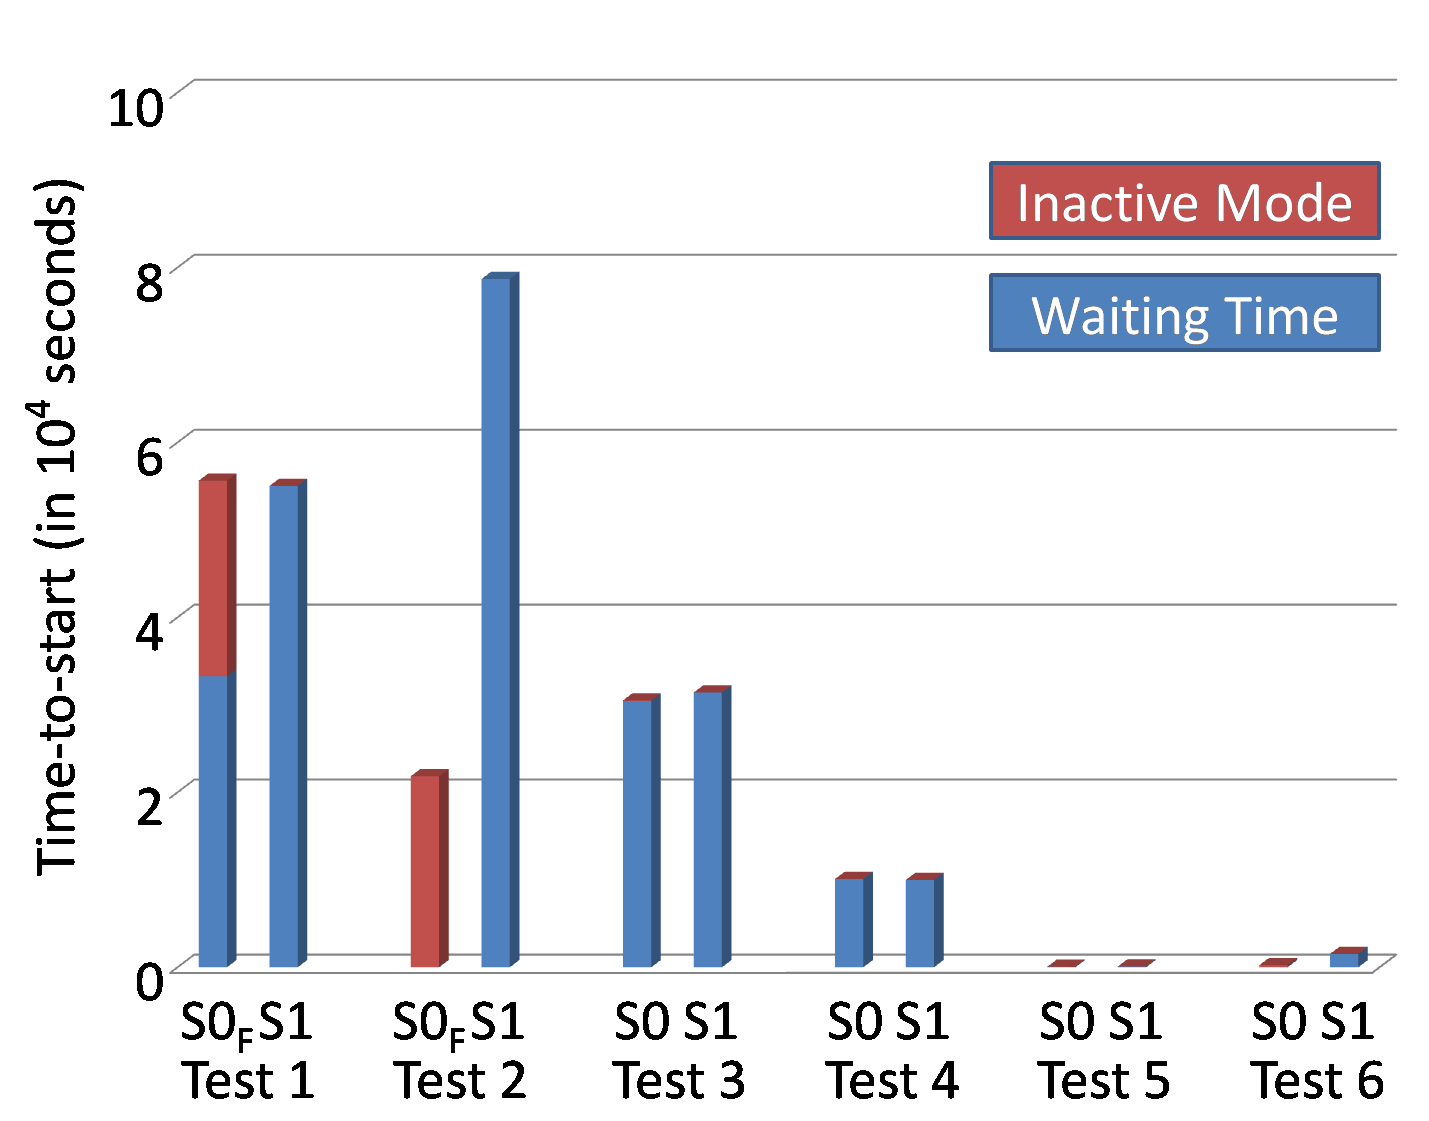
\includegraphics[scale=0.22]{Waiting_Clusters_6Hrs}
\linebreak
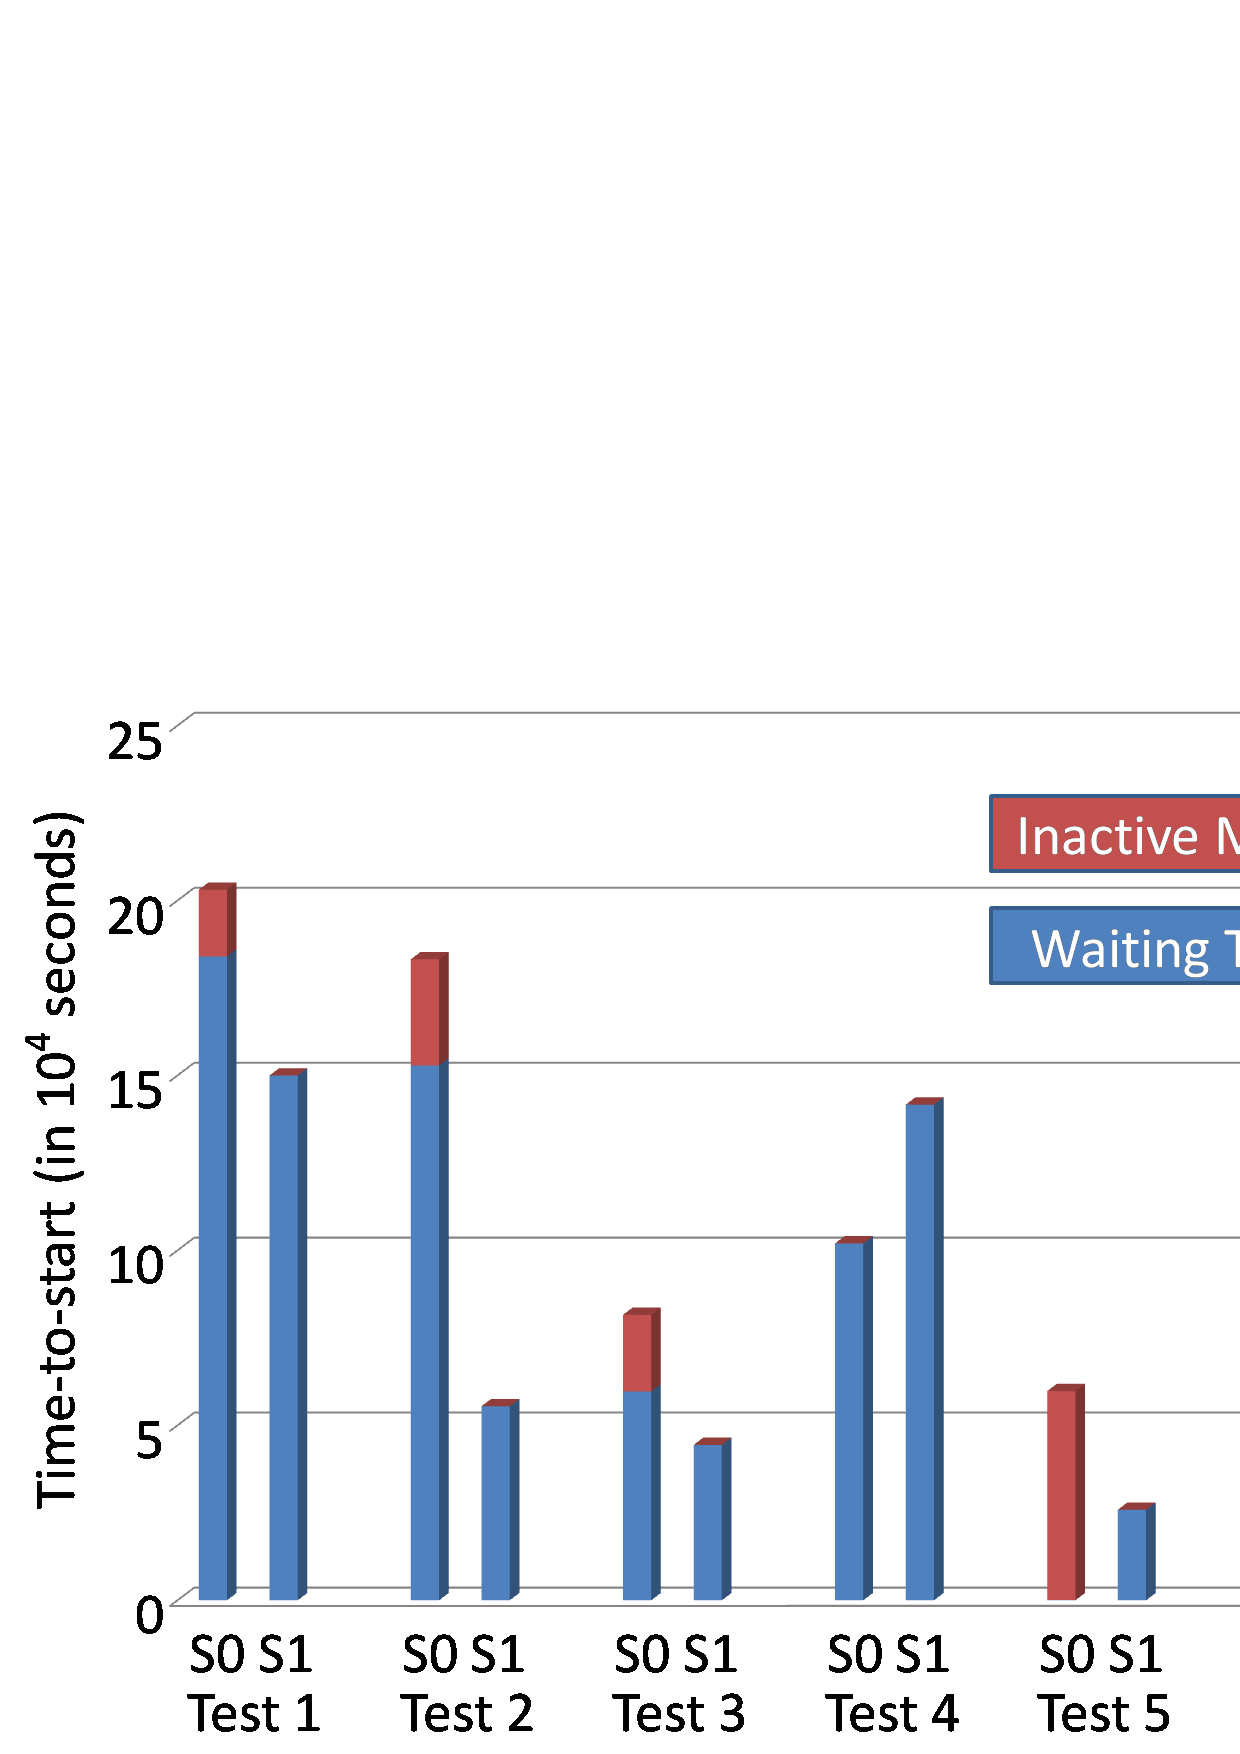
\includegraphics[scale=0.22]{Waiting_Clusters_24Hrs}
\caption{\small Waiting and inactive time for S0 (conventional job submissions) and S1 (a single BigJob submission), with the wall-time limit of 6 hours (upper graph) and 24 hours (lower graph). In both cases, S0 is submitted to use 2$\times$32 px and S1 requests 64 px on small and less crowded LONI clusters. Of 6 distinct experiments in each wall-time limit configuration, S1 showed faster time-to-start (i.e., the sum of waiting time and inactive mode) by 4 times in upper test and 5 in lower test; S0 even showed 2+1 failures to start the simulation due to the timeover \Nkimnote{time-over ??} of wall-time limit in the first-started job, denoted by $S0_F$.}
\label{Fig:BJwaiting}
\vspace{-1em}
\end{figure}
%%%%% FIGURE %%%%%


Results for smaller systems ($\approx$ 500 px) are presented in a different fashion in Fig.~\ref{Fig:BJwaiting}. In addition to the fact that a 64 px BigJob is now around 16\% of the machine resources, the load-factors of the smaller machines fluctuated much more than those of the larger machines. Consequently the data obtained for smaller resources is very noisy. As can be seen from Fig.~\ref{Fig:BJwaiting} although the waiting time for the first-to-start job was smaller in the conventional job submission (S0) than the BigJob (S1), the second job in S0 had a large subsequent waiting time; thus for conventional job submission mode there is a non-negligible inactive mode (defined as the time difference between queue wait times between the two simulations). There is no inactive mode for BigJob submission as by definition both simulations begin concurrently. Interestingly, a number of experiments failed to start the simulation, when the waiting time of the second job is greater than the wall-clock limit for the first-to-start job. In other words, the second job is still waiting on the queue in the duration that the first-to-start job is in active/run mode. This is typically alleviated with co-allocation of resources; however the number of production grid infrastructure that provide co-allocation (and co-scheduling) as a production service is very limited. This leads us to the heart of the advantage of the BigJob submission mode: circumventing the requirements of co-scheduling by providing an application level solution that preserves performance and guarantees non-failure due to large-fluctuations in queue waiting times. As we increase the wall-time limit, S1 is more likely to start faster than S0 and the failure to start the simulation in S0 tends to decrease.




\subsection{Scenario S1: Pilot-Job with Load Balancing}

Runtimes of the coupled simulation with a single BigJob is given on
Table~\ref{table:oneBJ_Test}. For both small and large simulations, a
default BigJob task takes about 1 percent longer than the conventional
test. This is reasonable because a default BigJob has the same
processor distribution between sub-jobs as the conventional job, while
BigJob has the minor overhead of sub-jobs' status monitoring and
communication with advert server. In cases of load-balanced BigJob
simulations, there is a significant reduction in the runtime compared
to successful conventional jobs -- 13\% and greater. For larger
problem set, a load-balanced BigJob simulation relatively shows higher
standard deviation (SD) due to the unexpected instability of a computing
resource during one experiment, to be discussed in detail
below.

\begin{table}[t]
%\setlength{\tabcolsep}{1pt}
%\begin{table}[!ht]
%\begin{center}
  \caption{\small Results of runtime for S1, $S1_{LB}$ and
    conventional submission. All measured times are in seconds and expressed as 'mean$\pm$SD'. 6 distinct experiments were accomplished
    for each simulation, all with 64 px. In both cases, S1 shows about 1\% overhead
    due to the communication with advert server. On the other hand,
    $S1_{LB}$ tests show about 13\% runtime save compared to
    conventional submission.}
\label{table:oneBJ_Test}
\centering
\begin{tabular} {p{0.5in} || p{0.7in} p{0.7in} p{0.7in}}
  \multicolumn{4}{c}{\phantom{\tiny 100}}\\
  \hline
  & \nyc Conventional
  & \nyc S1
  & \multicolumn{1}{c}{$S1_{LB}$}
  \\
  \hline
  \nyc Small sim. & \nyc 757$\pm$1.6 & \nyc 764$\pm$1.0 & \multicolumn{1}{c}{661$\pm$4.0} \\
  \nyc Large sim. & \nyc 39595$\pm$106.7 & \nyc 39906$\pm$178.7 & \multicolumn{1}{c}{34350$\pm$1189.2} \\
  \hline
%\midrule
\end{tabular}
\vspace{-1em}
\end{table}

The validity of a load balancing function can be discussed by the
change of processor distribution between subtasks throughout the
simulation. For the result of a small simulation in
Fig.~\ref{Fig:LBSmall}, both CFD and MD subtasks are assigned with 32
px initially. After two simulation loops, a load balancer
converges to the processor distribution of 12 to 52 px between
CFD and MD respectively; this processor distribution remains the same
until the simulation completes. Runtime per loop is reduced from 153
sec for the first loop to 107 sec after the convergence. Total
computation time is 596.19 sec, which is different from 663
sec counted from BigJob application manager. This time difference
implies that the BigJob application manager spends about 13 sec
per stage in executing its internal commands including the run of a
load balancing function and sub-job re-launch. % \jhanote{I don't see
%   how this is 13seconds saving? I can't see what the numbers 596 and
%   663s represent??}

%%%%% FIGURE %%%%%
\begin{figure}
%\vspace{-1em}
\centering
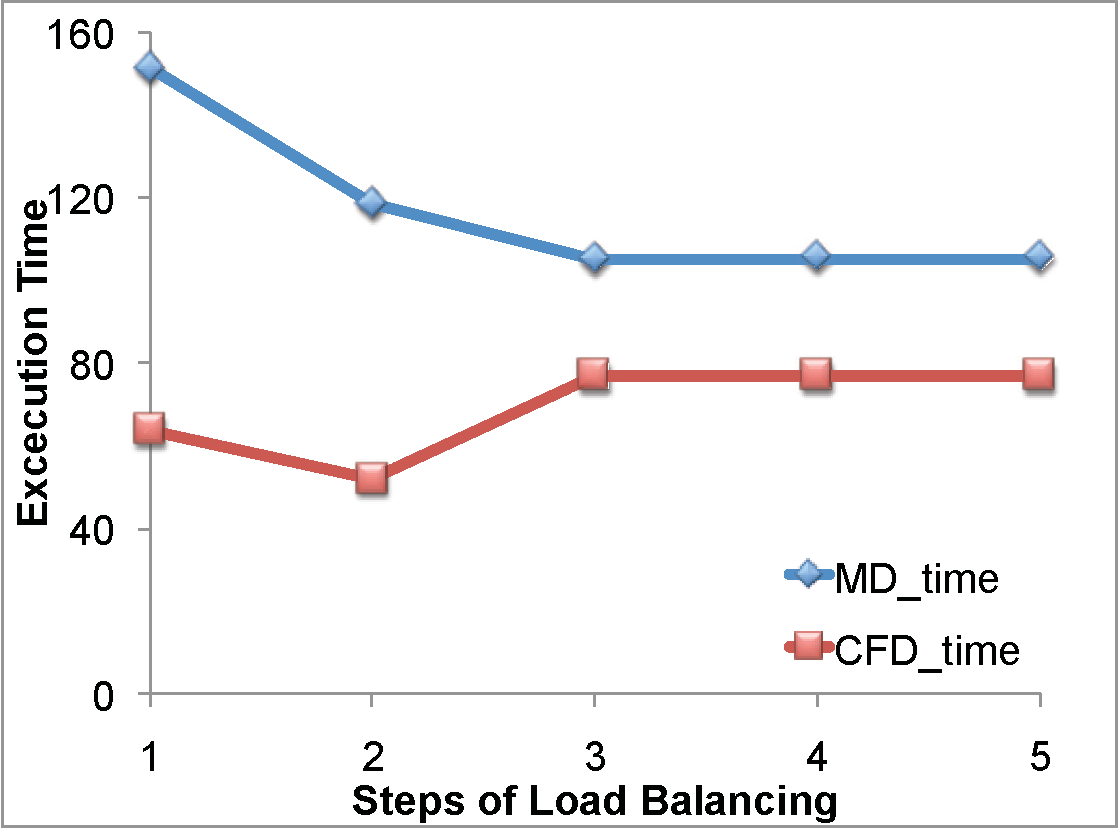
\includegraphics[scale=0.3]{fig6_1}
\linebreak
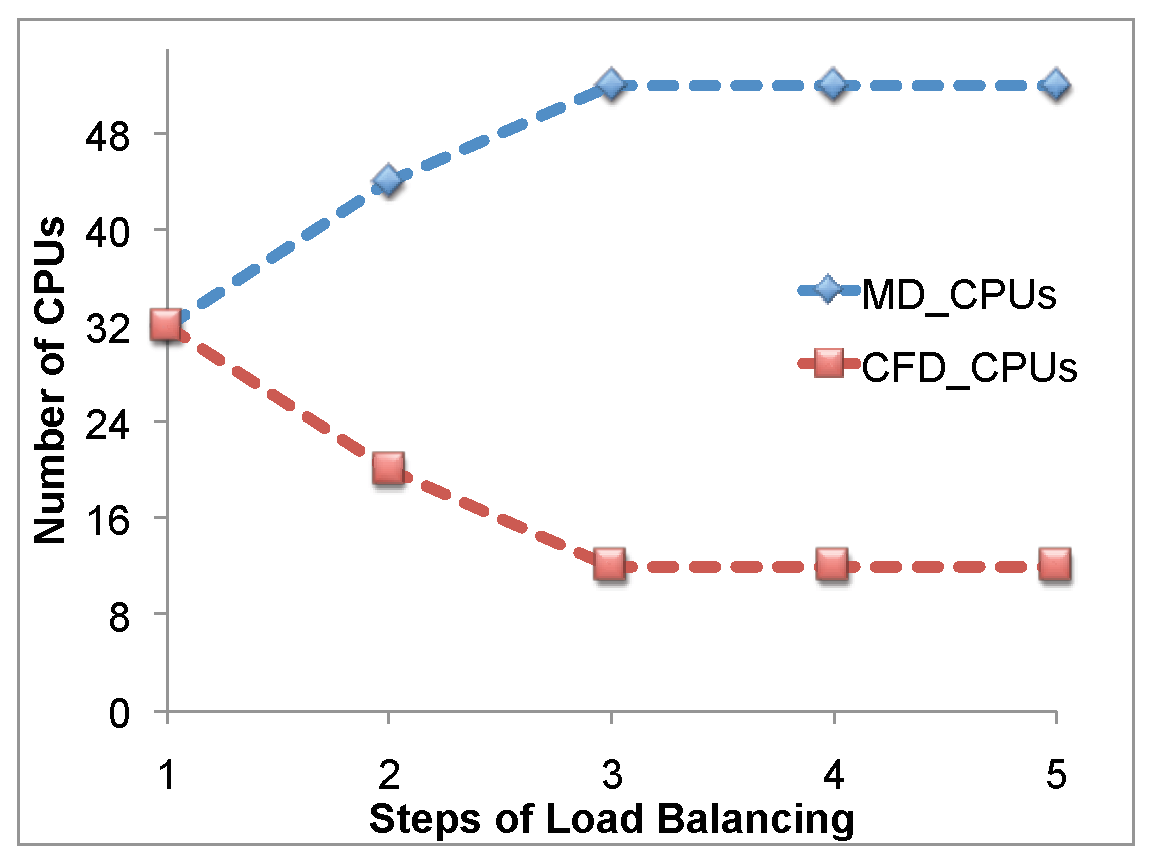
\includegraphics[scale=0.3]{fig6_2}
\caption{\small Change of processor distribution between CFD and MD
  jobs and resultant computation time in the small simulation. A load
  balancer starts from the same number of processors assigned to both
  sub-jobs and detects 20 to 44 px between each sub-job as the optimal
  solution. The poor scalability of CFD job makes the load balancer to
  search for the optimal condition once again and the processor
  assignment finally reaches to a steady solution of 12 to 52 between
  two sub-jobs. Computation time for every simulation loop reduces
  from 153 sec to 107 sec after the balancing.}
\label{Fig:LBSmall}
\vspace{-1em}
\end{figure}
%%%%% FIGURE %%%%%


The result of computation time evolution for a large simulation is
seen in Fig.~\ref{Fig:LBLarge}. For most experiments, which is given in
the left side of Fig.~\ref{Fig:LBLarge}, a load balancer directly goes
to a converged solution of processor distribution, which is 24 to 40
between CFD and MD jobs. On the other, in one experiment, computing
nodes assigned to MD simulation seem to have temporarily experienced
the internal overhead as shown from the right side of
Fig.~\ref{Fig:LBLarge}. This overhead temporarily increased MD
computation time a lot and a load balancer shows the fluctuating
pattern of processor distribution in response to this temporary
instability. A load balancer goes to a different steady solution after
the system settled down, which is the processor distribution of 20 to
44 between two sub-jobs. Compared to the steady solution in stable
cases, computation time for one simulation loop increases in this
processor distribution increases from 1320 sec to 1380
sec. % This leaves the requirement of refining a load balancing
% function, to predict more precisely on parallel performances of
% application codes.
Plots on the right side of Fig.~\ref{Fig:LBLarge} show a
non-monotonically changing resource assignment by the LB, and thus
demonstrating how the load balancer can be self-correcting and adapt
to changing performance; after increasing the number of processors
assigned to the MD, the load-balancer unassigns the additional
processors.


% %%%%% FIGURE %%%%%
\begin{figure}
%\vspace{-1em}
\centering
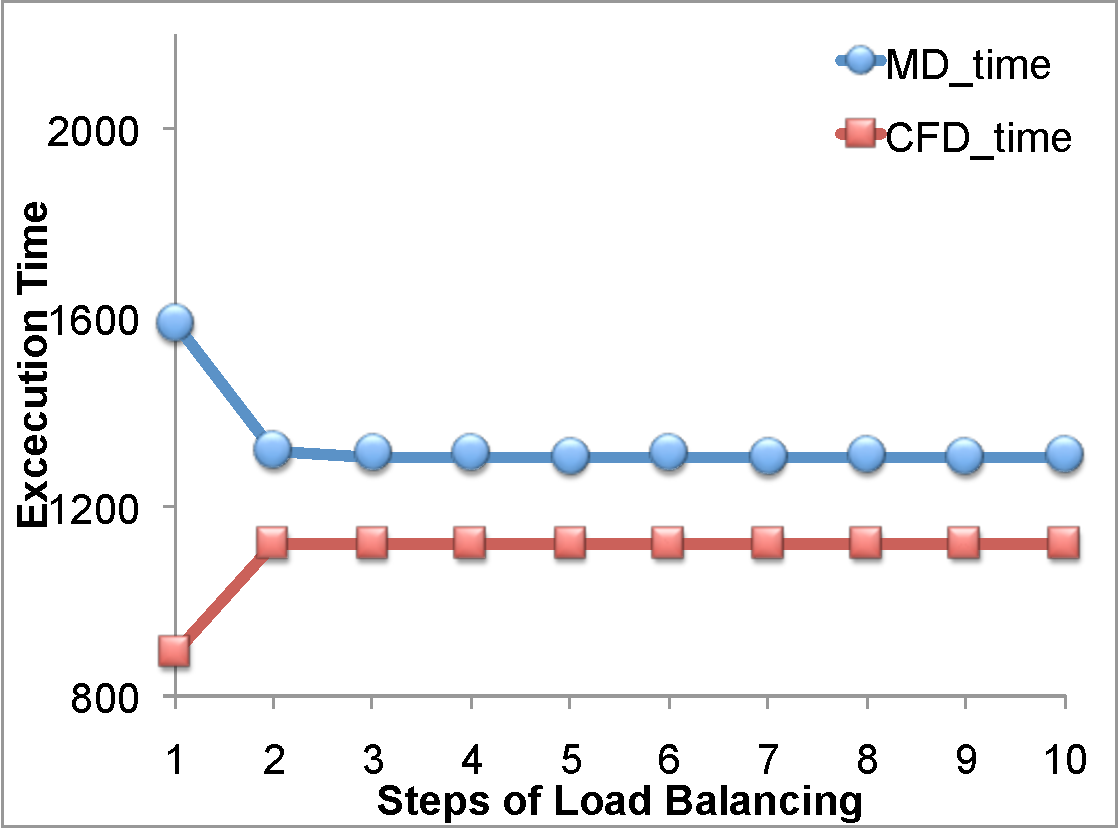
\includegraphics[scale=0.21]{fig7_11}
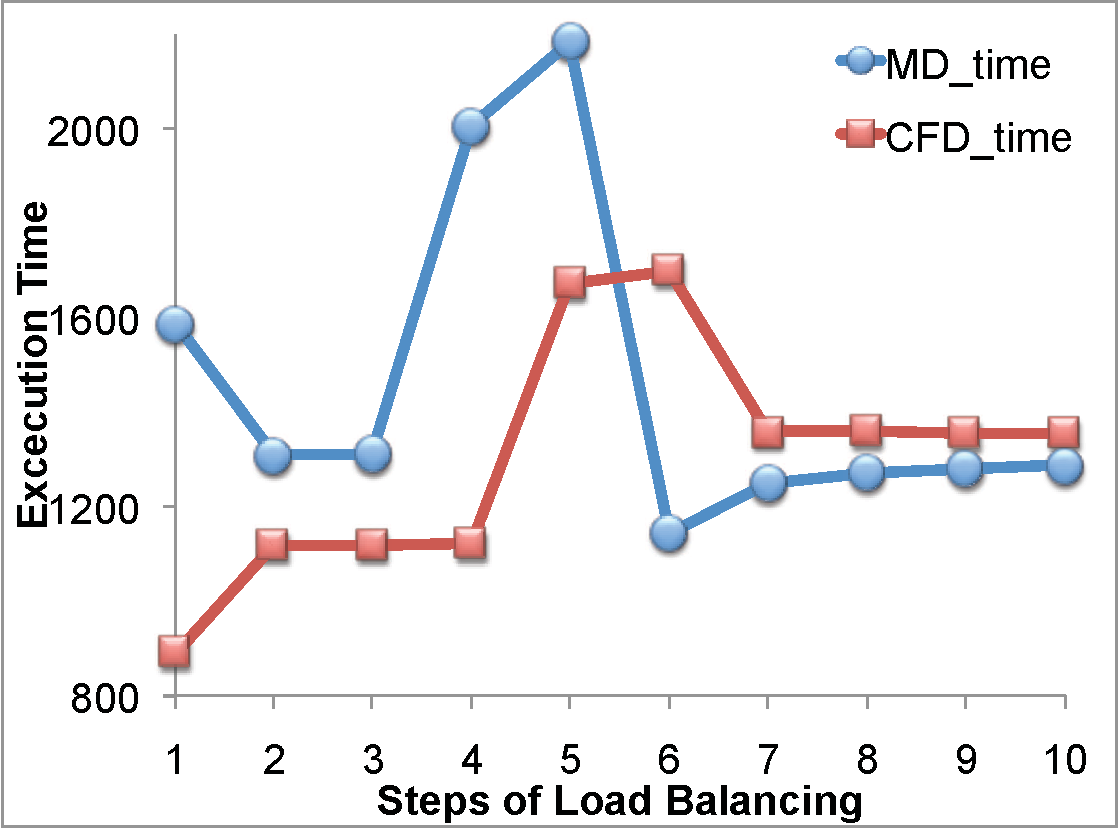
\includegraphics[scale=0.21]{fig7_21}
\linebreak
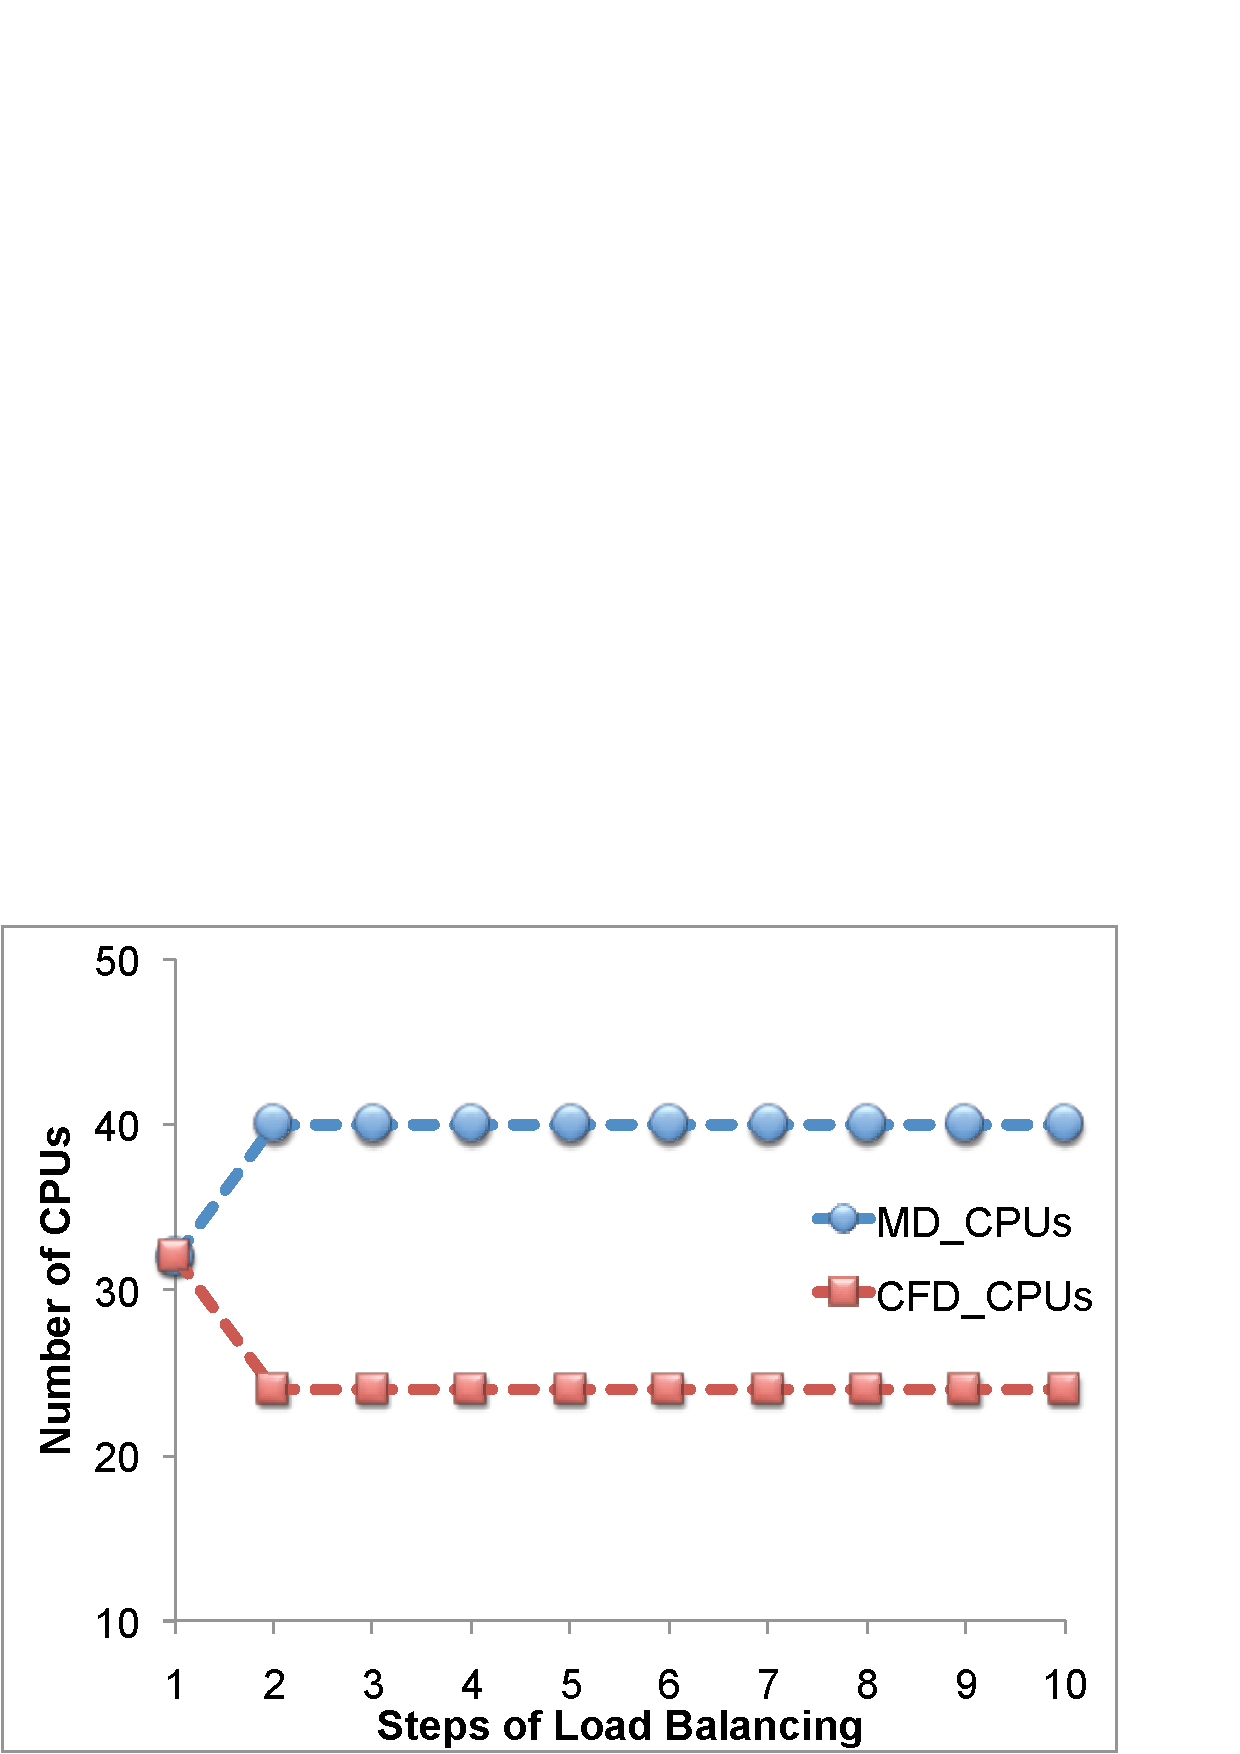
\includegraphics[scale=0.21]{fig7_12}
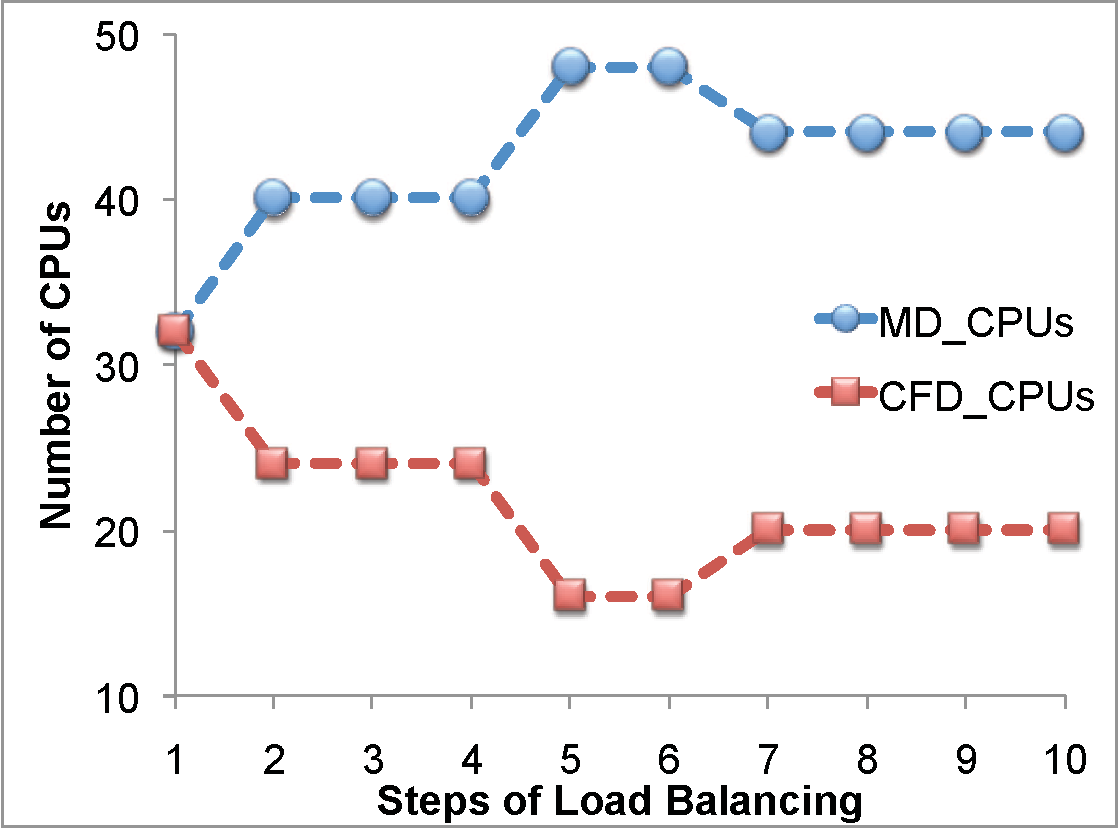
\includegraphics[scale=0.21]{fig7_22}
\caption{\small (Left Column) Change of processor distribution between
  CFD and MD jobs and resultant computation time in the large
  simulation. A load balancer directly finds the processor
  distribution of 24 to 40 between CFD and MD jobs and remains the
  steady state until it completes after 25 simulation loops. Initial
  computation time of 1605 sec reduces to 1320 sec after the
  convergence. (Right Column) Plots showing non-monotonic resource
  assignment by the LB, and thus demonstrating how the load balancer
  can be self-correcting and adapt to changing performance; after
  increasing the number of processors assigned to the MD, the
  load-balancer unassigns the additional processors.}
\label{Fig:LBLarge}
\vspace{-1em}
\end{figure}
%%%%% FIGURE %%%%%


%\jhanote{You need to really sit down and rewrite this. It is almost
%  impossible to understand anything here!!!}


\subsection{Scenario S2 and S3: Logically and Physically Distributed
  Pilot-Jobs}

In Table~\ref{table:TwoBigJobs}, results from the four test runs
representing scenarios S2 and S3 using two BigJobs are presented.  The
general setup for scenarios S2 and S3 is that when two BigJobs are
submitted, one BigJob becomes active first and the other BigJob
becomes available later -- either on the same resource (S2) or on
another resource (S3).  The MD and CFD request half of each
BigJob. When the second BigJob becomes active, each application is
immediately configured to run in each BigJob so as to consume all
BigJob CPUs. Therefore, more CPUs allow each application to speed
up. Conceptually the LB scheme adopted for S1 can be trivially applied
here, but for simplicity and as proof-of-concept, we confine our test
runs to the configuration in Fig.~\ref{Fig:TwoBigJobs}, i.e., without
a load balancing scheme to determine an optimal distribution of
resources.

% \jhanote{I think
%       we should revisit the way this is presented, i.e., the utility
%       of using the time of the MD phase?}  \Jkimnote{I got rid of MD
%       time as a measure since it causes unnecessary confusion}
%     \jhanote{this caption is tooooo long and needs simplifying. Too
%       many latex errors!} \jhanote{Look at all the wasted white
%       space!!! We are running short of space. Fix}

\begin{table}[!h]
\begin{center}
  \caption{\small Performance measured for Scenarios S2 and S3 (2
    BigJobs on 2 different machines).  Here, we present the time to
    solution in terms of two components, ${T_{comm}}$ and
   ${T_{compute}}$.  The details on how to conduct these experiments
    are described in the text.  All measured time are in seconds.
    BigJob size refers to the size of two BigJobs as determined by the
    number of requested cpus \Nkimnote{CPUs}. Resource describes the system used (L
    stands for Louie; P for Poseidon. L \& P are LONI resources) }
\label{table:TwoBigJobs}
\begin{tabular}{ c || c  c  c  c}
  \multicolumn{5}{c}{\phantom{\tiny 100}}\\
\hline
Test & 1 & 2 & 3 & 4  \\

\hline
Scenario & S2 & S2 & S3 & S3 \\
BigJob size & (8,16)  & (8,16) & (8, 16) & (16,32) \\
Resource & P  & L  &  L + P & L + P \\
\hline
1 BigJob &   & & & \\
${T_{compute}}$ & 1037.2& 1045.2 & 1049.0 & 534.2\\
${T_{comm}}$ & 0.006 & 0.010 & 0.912 & 0.957 \\
\hline
2 BigJob  &   & & & \\
${T_{compute}}$ & 277.2 & 277.8& 276.8 & 150.4 \\
${T_{comm}}$ & 0.041 & 0.009 &  0.990 & 0.60 \\
\hline
\end{tabular}
\end{center}
\end{table}
% \jhanote{The $T_{comm}$ has two components: $T_{read_write} +
%   T_{transfer}$. We need to determine the first component. We will not
%   be able to do so rigorously, but we need to show a good-faithed
%   attempt at deriving it.  The we need to determine the transfer
%   overheard, and find out if it is truly negligible when compared to
%   $T_{read_write}$. We need to also mention/determine if
%   $T_{read_write}$ is the same -- when using 2 different machines as
%   it is when using 1 machine. As would be expected.}

As shown in the table, the results with these four test cases clearly
demonstrate performance gains with additionally available cpus when
two BigJobs.  The performance gain is examined with respect to two
components ${T_{comm}}$ and ${T_{compute}}$ of the total
time-to-solution.  % The major performance gain is indicated with a
% shorten ${T_{compute}}$.
${T_{compute}}$ represents the maximum of (${T _{MD,compute}}$,
${T_{CFD,compute}}$) -- which is the longer compute time of two
applications, and%  Each $T_{app,compute}$, where ${app}$ is MD or CFD, is
% measured with
by the start time and the end time between the data exchange.  As more
cpus become available with the incoming BigJob, more gain in the
performance is achieved as shown in the case of test 4.  On the other
hand, the time for communication, ${T_{comm}}$ is further decomposed
into ${T_{read-write}}$ and ${T_{file-transfer}}$.  Note that the
latter is only required with S3.  There are other components that
contribute to the overall time-to-solution, such as the waiting time
in queue etc., but are not considered here to focus on the performance
gain arising from simple dynamic execution (resource allocation) as
illustrated from S2 and S3.

% Performance gains with two BigJobs. Performance is measured with CPU
% times consumed by MD, since test cases we used always require longer
% CPU times for MD than those of CFD.  Performance gains with
% additionally available BigJob can be seen by comparing MD CPU times
% with those obtained with the initial BigJob.  Measurements were
% carried out with LONI cluster systems.  louie and poseidon are dell
% cluster systems having 128 nodes with 4 cores in a
% node. \jhanote{add BigJob size --- which 8 and 16} Test 1 and 2
% correspond to Use Case 2; Test 3 and 4 correspond to Use Case 3
% \newline }

According to our results, the communication time is insignificant even
for S3 --  thanks in part to the small size of the data required to be
exchanged.  Of course, the file transfer depends heavily on the
network condition, but it is not expected to become a major issue
considering the observation that ${T_{comm}}$ is a tiny fraction of
${T_{compute}}$.  Furthermore, we expect that the ratio of the two
components will remain similar, or if anything becomes larger (i.e.,
${T_{comm}}$ becomes less significant) as the size of physical system
simulated increases, i.e., the number of particles in MD or the number
of mesh points increases.  Indeed, the development of an efficient
runtime environment for hybrid CFD/MD simulation lies in finding a way
to decrease ${T_{compute}}$.  Arguably, the results in the
table~\ref{table:TwoBigJobs} suggest that a BigJob-based runtime
environment is able to provide a reasonable solution to this end.

\section{Conclusions}


In this work, we report the first production application-level
framework that uses generalizations of the Pilot-Job to enable an
efficient runtime environment targeting coupled multi-physics
application comprising MD and CFD.  It is not trivial to integrate a
targeted scientific application with a resource management system that
is aware of the challenges arising from the distribution -- logical
and/or physical, well as the local scheduler implemented with the
local resource management policy.  Overcoming the co-scheduling
requirements and implementing dynamic resource allocation mechanism
were two main goals motivating a novel development and our test runs
demonstrated its potential for large scale scientific simulations
benefiting scientific problems that are only tackled by a coupled
hybrid MD-CFD calculation.  Our development is built upon the BigJob
framework enabled by the SAGA which provides a simple and consistent
interface for managing HPC resources and natively supports an agile
and flexible execution model.

We validated and tested development for performance on three cases and
demonstrated its capability.  Our approach is minimally intrusive
towards the application code.  Using MPI as a coupling layer would
also require code modification, adding infrastructure to support
simulation-to-simulation communication. To maintain a high level of
adaptivity, abstraction, interoperate between various application
codes, and to eliminate application code invasion, we opted not to use
MPI and focus on non-invasive abstract coupling layers.  Some of these
problems arise from the nature of the simulations: large scale
simulations that would not be able to run concurrently on the same
resource, while others issues are quite technical such as dynamic
shrinking/expanding the number of MPI processes of each application
(dynamic load-balancing).

In summary, we have established that the use of a BigJob as a
container for coupled-simulations is an effective approach. Not only
is runtime performance preserved, but in the absence of production
grade co-scheduling/co-allocation service, there is a significant
reduction in the waiting time and a complete elimination of failed
runs due to excessive long queue waiting times.  Also, the BigJob
framework supports the use of a load balancing function, which enables
coupled codes to use the allocated resources more efficiently. We have
established that the performance advantage of using BigJobs is
invariant with the size of the machine, i.e., small LONI machines such
as Eric, to the largest machines available such as Ranger. This claim
is valid not only as machines get larger, but also for progressively
larger physical models that we are investigating. We will report
results on these in the near future.

% Meanwhile, launch of two BigJobs does not intend to use resources more
% efficiently than conventional job allocation, but intend to save total
% computation time more than one BigJob test case, by utilizing more
% available resources.




% In addition, the use cases includes the usage of the Condor-glide-in
% as our BigJob framework is closely related. ... Some of those are i)
% employment of load balancing mechanism ii) advantages from
% implementation of dynamic allocation in heterogeneous distributed
% computing resources iii) simple solution for the co-scheduling
% requirements for the coupled tasks.

 % \jhanote{Notes: (i) (ii) Need to establish clearly how we are
  %   measuring the times in Table I. Are we using 'startq'? Remember
  %   enough details should be presented to make the experiments
  %   reproducible (iii) What is the largest system size that we can
  %   simulate using BigJob and/or using independent execution
  %   threads? (iv) What is the final ratio of $N_{MD} to N_{CFD}$? Is
  %   it always the same? How do we counter the argument that the
  %   final configuration can be determined with a few simple
  %   pre-processing runs? What is the importance of dynamic resource
  %   management, i.e. start with initial Configuration I and adapt to
  %   Final Configuration F with intermediate states in between?  }


\section*{Acknowledgment}
This work is part of the Cybertools (http://cybertools .loni.org)
project and primarily funded by NSF/LEQSF (2007-10)-CyberRII-01.
Important funding for SAGA has been provided by the UK EPSRC grant
number GR/D0766171/1 (via OMII-UK). This work has also been made
possible thanks to computer resources provided by LONI. We thank Andre
Luckow for initial work on BigJob, Lukasz Lacinski for help with SAGA
deployment (via HPCOPS NSF-OCI 0710874) and Joao Abecasis for his work
on the SAGA Condor adaptors.

%-------------------------------------------------------------------------
\nocite{ex1,ex2}
%\bibliographystyle{latex8}
\bibliographystyle{IEEEtran}
\bibliography{saga_tg08}


\end{document}


